\documentclass[12pt,a4paper]{article}
 
\usepackage{float}
%für feststellen der figures und tables [H] dranschreiben
\usepackage{units}
%wird so benutzt: 
%\unit[value/Zahl]{dimension/Einheit} oder 
%\unitfrac[value/Zahl]{dimension/Einheit num/Zähler}{dimension/Einheit denum/Nenner} oder
%\nicefrac[fontcommand/Schriftart]{dimension/Einheit num/Zähler}{dimension/Einheit denum/Nenner}

\usepackage{caption}
\usepackage{subcaption}

\usepackage{hyperref}

\usepackage[left=2cm,right=2cm,top=2cm,bottom=2cm]{geometry}
\usepackage[utf8]{inputenc}
\usepackage[T1]{fontenc}
\usepackage{lmodern}
\usepackage[ngerman]{babel}
\usepackage{amsmath}
\usepackage{graphicx}
 
%niemals zwei überschriften direkt übereinander schreiben, also immer mindestens in einem satz was sinnvolles unter jede überschrift schreiben (bei den versuchen z.B. das versuchsziel) 
\begin{document}
%deckblatt erstellen.


\begin{titlepage}

\begin{center}
% Oberer Teil der Titelseite:

\includegraphics[width=0.75\textwidth]{logo.pdf}\\[1cm]    	%Logo 

\textsc{\LARGE Bergische Universität Wuppertal}\\[1.5cm]	%Institution

\textsc{\Large Elektronik Praktikum}\\[0.5cm]				%Projekt


\newcommand{\HRule}{\rule{\linewidth}{0.5mm}}
\HRule \\[0.4cm]
{ \huge \bfseries Datenerfassung mit dem Computer}\\[0.4cm]				%Titel

\HRule \\[1.5cm]

% Author und Tutor
\begin{minipage}{0.4\textwidth}
\begin{flushleft} \large
\emph{Autoren:}\\
Henrik \textsc{Jürgens} \\
Frederik \textsc{Strothmann}
\end{flushleft}
\end{minipage}
\hfill
\begin{minipage}{0.4\textwidth}
\begin{flushright} \large
\emph{Tutoren:} \\
Hans-Peter \textsc{Kind} \\
Peter \textsc{Knieling} \\
Marius \textsc{Wensing}
\end{flushright}
\end{minipage}

\vfill

% Unterer Teil der Seite/Datum
{\large \today}

\end{center}

\end{titlepage}

\newpage
\tableofcontents
\newpage
\section{Einleitung}
%einleitung zu dem experiment.
%auf die einstellungen, die vor dem versuch gemacht werden, eingehen oder auf eine anleitung dazu verweisen
%es soll immer erwähnt werden um was es in dem Versuch geht und wie das relisiert werden soll
%---------------------------------------------------------------------------------------------
%hinter der einleitung kann der allgemeine theoretische hintergrund in einer zusätzlichen section erklärt werden
%1-----------------------------------------------1

Dieser Versuch beschäftigt sich mit den Fragestellungen, wie man digitale in analoge Signale umwandelt, wie ein Computer kontinuierliche Spannungswerte erzeugen kann, wie analoge Werte digitalisiert werden können, wie ein Digitalvoltmeter kontinuierliche Spannungswerte erfassen und digital anzeigen kann und wie sich Zeiten oder Frequenzen messen lassen.

\section{Umwandlung digitaler in analoge Signale, DAC}
%kurz das ziel dieses versuchsteiles ansprechen, damit keine zwei überschriften direkt übereinander stehen!
%bei schwierigeren versuchen kann auch der theoretische hintergrund erläutert werden. (mit formeln, herleitungen und erklärungen)

In diesem Versuchsabschnitt werden verschiedene Digital-Analog-Converter gebaut und untersucht. Realisiert werden der Digital-Analog-Converter mit einem Binär- und einem R-2R-Netzwerk. 

\subsection{DAC mit binärem Netzwerk}
%kurz das ziel dieses versuchsteiles ansprechen, damit keine zwei überschriften direkt übereinander stehen!
%bei schwierigeren versuchen kann auch der theoretische hintergrund erläutert werden. (mit formeln, herleitungen und erklärungen)

In diesem Versuchsteil wird ein DAC mit einem Binärnetzwerk aufgebaut. Der Nachteil dieses Aufbaus ist, dass für hohe Auflösungen genaue Widerstände benötigt werden. Die Auflösung bestimmt sich mit:
\begin{align}
\text{U}_\text{A}=\text{U}_0 \cdot \frac{\text{Binärwert}}{2^\text{n}-1}
\label{eqn:binaer}
\end{align}

\subsubsection*{Verwendete Geräte}
%(immer) eine skizze oder ein foto einfügen, die geräte/materialien !nummerieren! und z.b. eine legende dazu schreiben, besser wäre es das ganze in einem Fließtext gut zu beschreiben.
%falls am anfang des versuches nicht klar ist, was alles verwendet wird, wenn möglich erst am ende ein großes foto von den verwendeten materialien machen!\\

Es werden das Versuchsboard, das Zusatzboard, ein PC, ein Steckaufsatz und eine $2^\text{n}$ Folge von Widerständen verwendet.

\subsubsection*{Versuchsaufbau}
%skizze zum versuchsaufbau (oder foto) einfügen,   es muss erklärt werden wie das ganze funktioniert und welche speziellen einstellungen verwendet wurden (z.b. welche knöpfe an den geräten für die messung verdreht wurden)

In Abbildung \ref{fig:auf_1_1} ist der Schaltplan eines ADCs mit binärem Widerstandsnetzwerk zu sehen. Die Schaltung wird mit dem Versuchsboard und einem Binärnetzwerk realisiert.

\begin{figure}[H] 
  \centering 	
    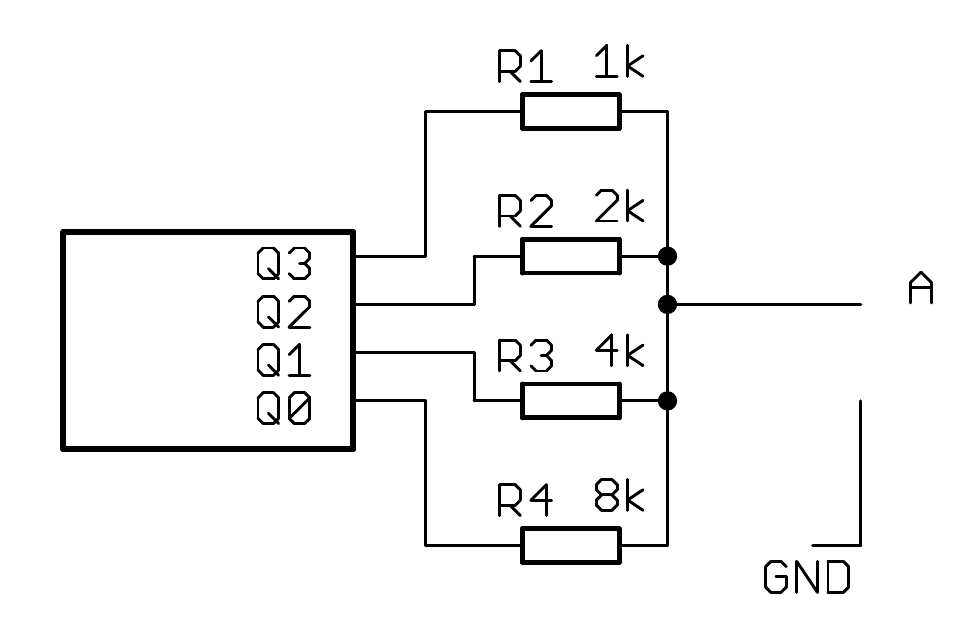
\includegraphics[ scale = 0.4]{auf_1_1.png}
  	\caption[Schaltplan für ein DAC mit binärem Widerstandsnetzwerk]{Schaltplan für ein DAC mit binärem Widerstandsnetzwerk\footnotemark}
  \label{fig:auf_1_1}
\end{figure}
\footnotetext{Abbildung entnommen von http://www.atlas.uni-wuppertal.de/$\sim$kind/ep11\_14.pdf am 18.01.2015}

\subsubsection*{Versuchsdurchführung}
%erklären, !was! wir machen, !warum! wir das machen und mit welchem ziel
%(wichtig) präzize erklären, wie bei dem versuch vorgegangen und was gemacht wurde

Der größte Widerstand wird an die erste Binärstelle angeschlossen und an jede weitere Binärstelle jeweils die Hälfte des vorherigen Widerstandes. Das Widerstandsnetzwerk wird auf das Versuchsboard gesetzt. Zuerst werden die ersten 4 Bits des Binärzählers verwendet und das Ausgangssignal mit dem Oszilloskop aufgenommen. Danach werden die ersten 8 Bits des Binärzählers verwendet und das Ausgangssignal mit dem Oszilloskop aufgenommen. Die Messung wird mit dem Befehl c gestartet. Der Mikrocontroller übernimmt in diesem Fall die Funktionen des Oszillators und des Binärzählers.

\subsubsection*{Auswertung}
%zuerst !alle! errechneten werte entweder in ganzen sätzen aufzählen, oder in tabellen (übersichtlicher) dargestellen, sowie auf die verwendeten formeln verweisen (die referenzierung der formel kann in der überschrift stehen)
%kurz erwähnen (vor der tabelle), warum wir das ganze ausrechnen bzw. was wir dort ausrechnen
%danach histogramme und plots erstellen, wobei wenn möglich funktionen durch die plots gelegt werden (zur not können auch splines benutzt werden, was aber angegeben werden muss)
%bei fits immer die funktion und das reduzierte chiquadrat mit angegeben, wobei auf verständlichkeit beim entziffern der zehnerpotenzen geachtet werden muss z.b. f(x)=(wert+-fehler)\cdot10^{irgendeine zahl}\cdot x + (wert+-fehler)\cdot10^{irgendeine zahl}
%bei jedem fit erklären, nach welchem zusammenhang gefittet wurde und warum!
%bei plots darauf achten, dass die achsenbeschriftung (auch die tics) die richtige größe haben und die legende im plot nicht die messwerte verdeckt
%kurz die aufgabenstellung abhandeln
%2-----------------------------------------------2

Erwartet wird eine Treppen-artiger Verlauf bei der Messung der Ausgangsspannung erwartet. Die Differenz zwischen zwei Stufen ergibt sich nach Gleichung \ref{eqn:binaer} mit $\frac{\text{U}_0}{2^\text{n}-1}$. Für die 4 Bits ergab sich der Verlauf in Abbildung \ref{fig:1_1_1}, die einzelnen Stufen sind deutlich zu sehen. Die Auflösung liegt bei einem fünfzentel.

\begin{figure}[H] 
  \centering 	
    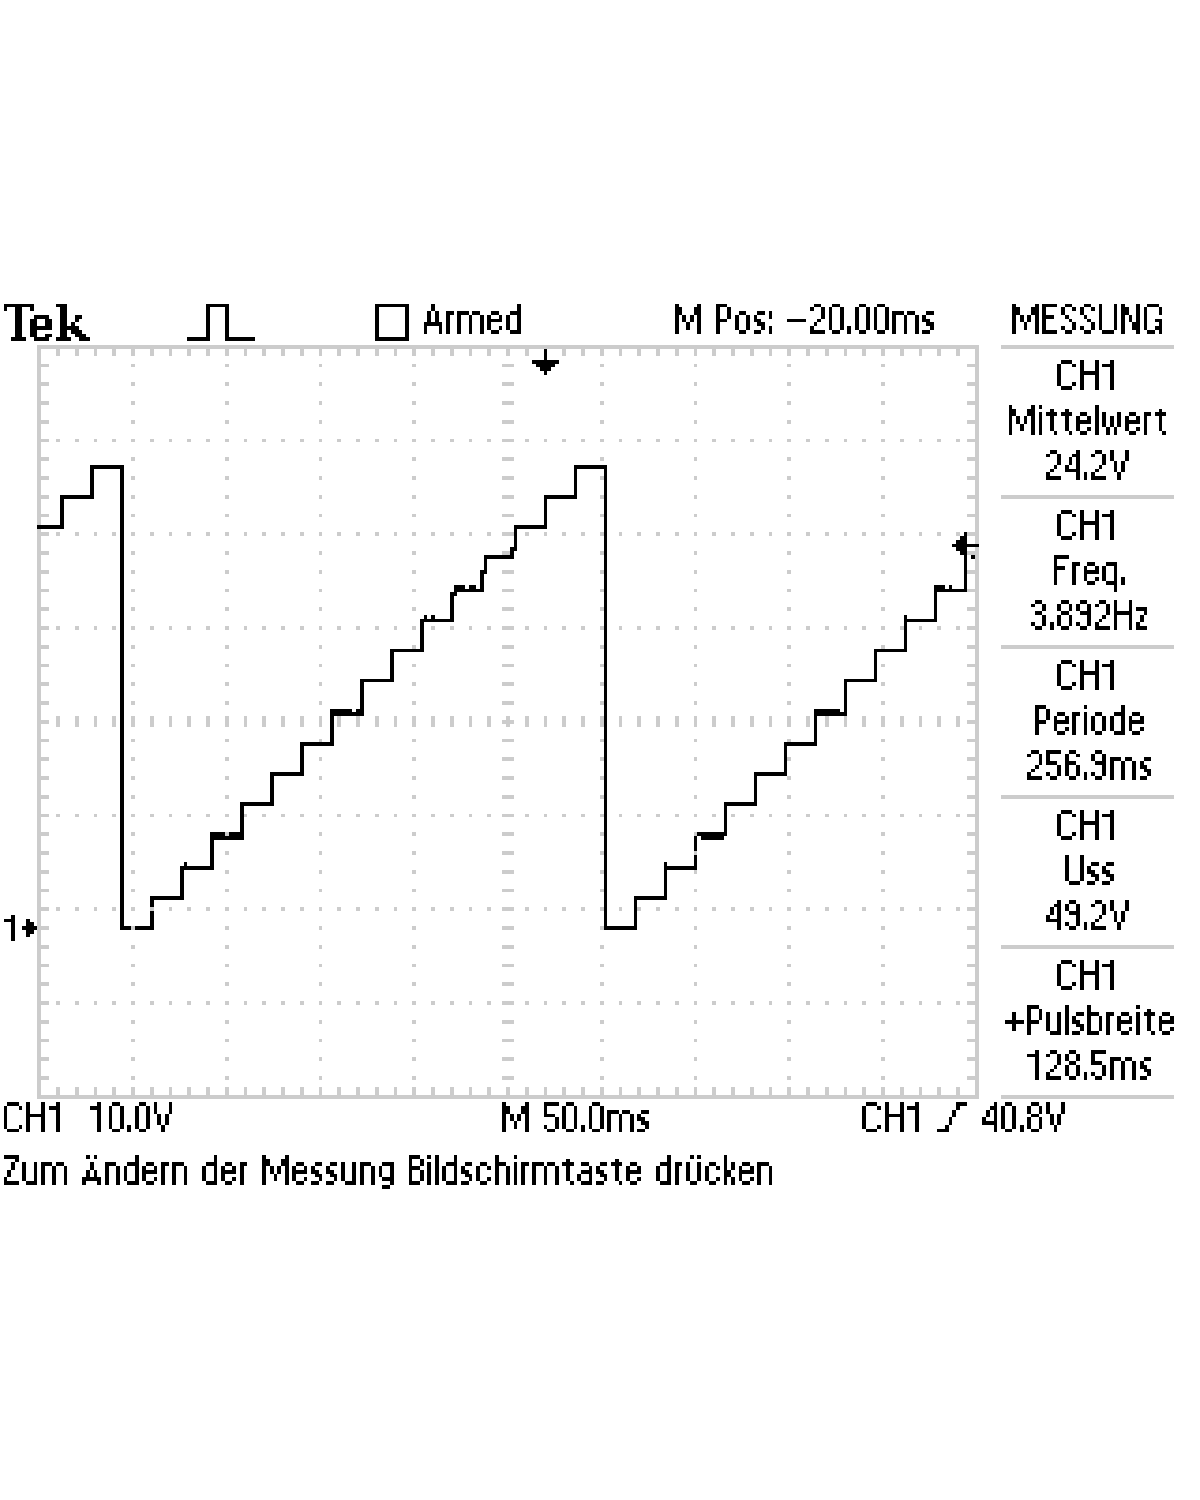
\includegraphics[trim = 0mm 50mm 0mm 50mm, clip, scale = 0.4]{1_1_1.pdf}
  	\caption[Aufnahme der Ausgangsspannung]{Aufnahme der Ausgangsspannung} 
  \label{fig:1_1_1}
\end{figure}

Die Aufnahme des Kurvenverlaufs für 8 Bit ist in Abbildung \ref{fig:1_1_2} zu sehen. Die Stufen sind nicht zu erkennen, dies liegt an der Auflösung, die bei einem 255-stel liegt.

\begin{figure}[H] 
  \centering 	
    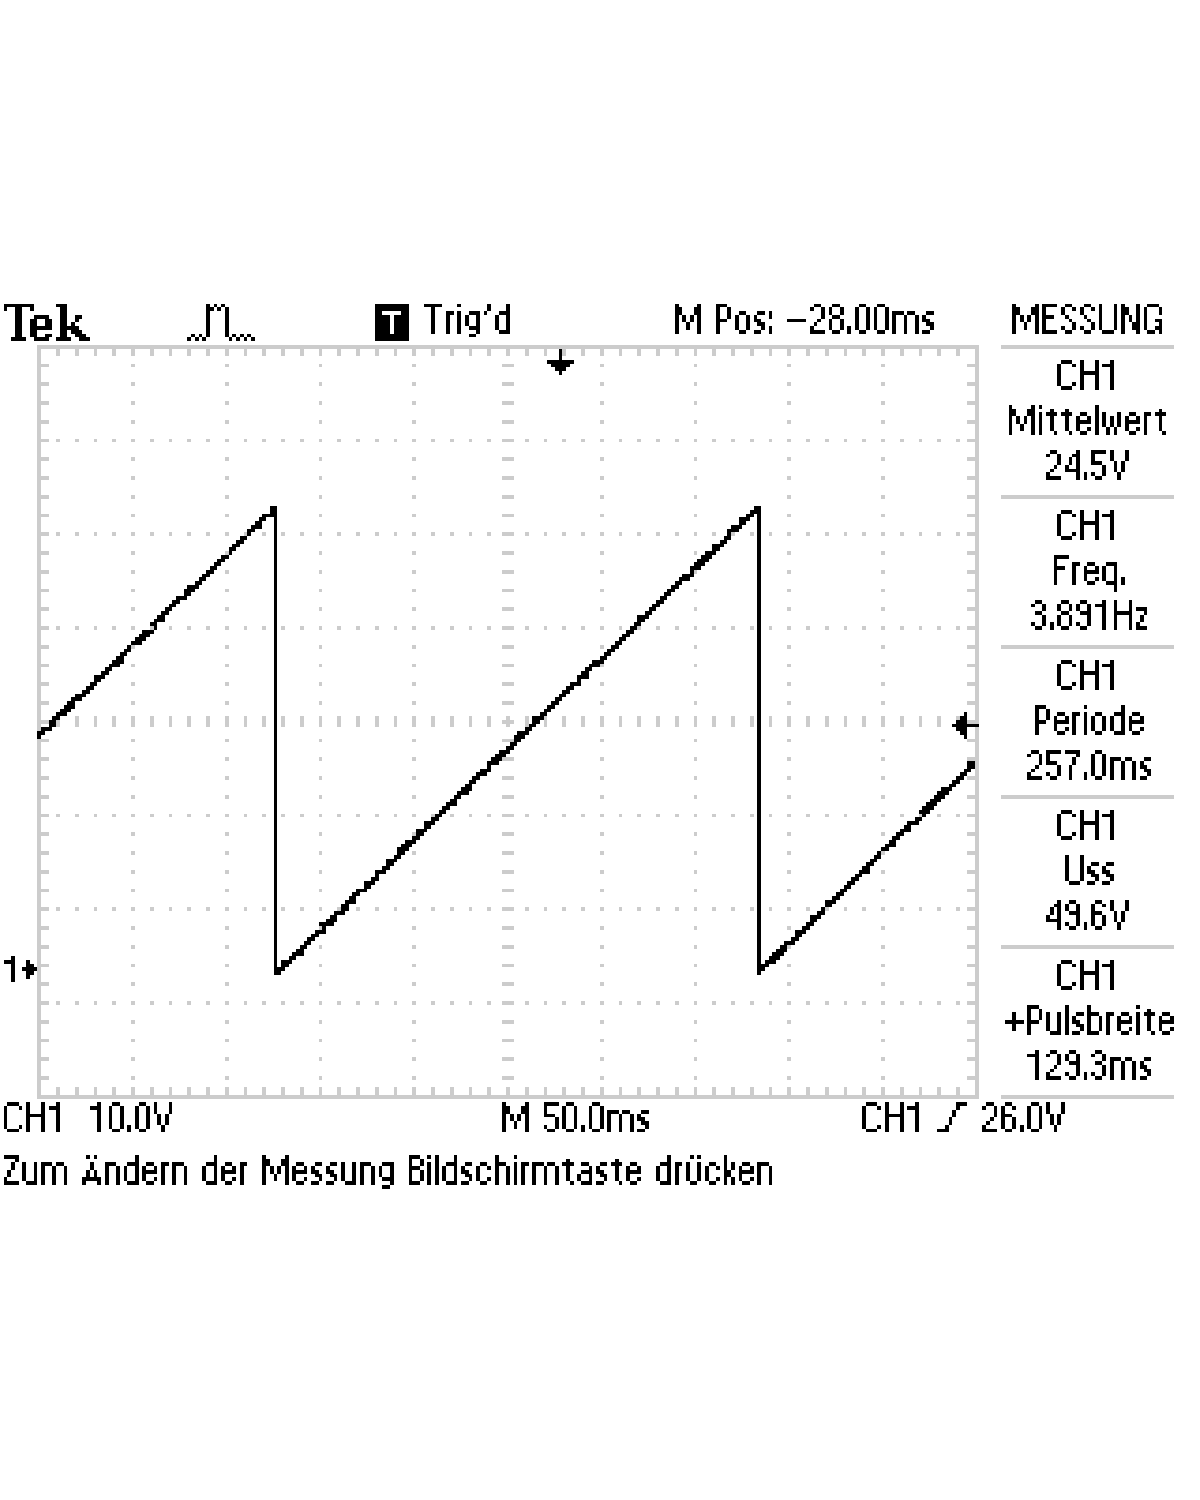
\includegraphics[trim = 0mm 50mm 0mm 50mm, clip, scale = 0.4]{1_1_2.pdf}
  	\caption[Aufnahme der Ausgangsspannung]{Aufnahme der Ausgangsspannung} 
  \label{fig:1_1_2}
\end{figure}



\subsection{DAC mit R-2R-Netzwerk}
%kurz das ziel dieses versuchsteiles ansprechen, damit keine zwei überschriften direkt übereinander stehen!
%bei schwierigeren versuchen kann auch der theoretische hintergrund erläutert werden. (mit formeln, herleitungen und erklärungen)

In diesem Versuchsteil wird ein DAC mit einem R-2R-Netzwerk untersucht. Der Vorteil diese Aufbaus ist, dass nur zwei verschieden Widerstände benötigt werden, die ein Verhältnis von 1:2 haben. Die Auflösung bestimmt sich mit:

\begin{align}
\text{U}_\text{A}=\text{U}_0 \cdot \frac{\text{Binärwert}}{2^\text{n}}
\label{eqn:binaer_2}
\end{align}

\subsubsection*{Verwendete Geräte}
%(immer) eine skizze oder ein foto einfügen, die geräte/materialien !nummerieren! und z.b. eine legende dazu schreiben, besser wäre es das ganze in einem Fließtext gut zu beschreiben.
%falls am anfang des versuches nicht klar ist, was alles verwendet wird, wenn möglich erst am ende ein großes foto von den verwendeten materialien machen!\\

Es werden das Versuchsboard, das Zusatzboard, ein PC, ein Steckaufsatz mit einem R-2R Widerstandsnetzwerk verwendet.

\subsubsection*{Versuchsaufbau}
%skizze zum versuchsaufbau (oder foto) einfügen,   es muss erklärt werden wie das ganze funktioniert und welche speziellen einstellungen verwendet wurden (z.b. welche knöpfe an den geräten für die messung verdreht wurden)

Der Schaltplan eines R-2R Netzwerkes ist in Abbildung \ref{fig:auf_1_2} zu sehen. So ein Netzwerk wird auf das Zusatzboard gesetzt.

\begin{figure}[H] 
  \centering
    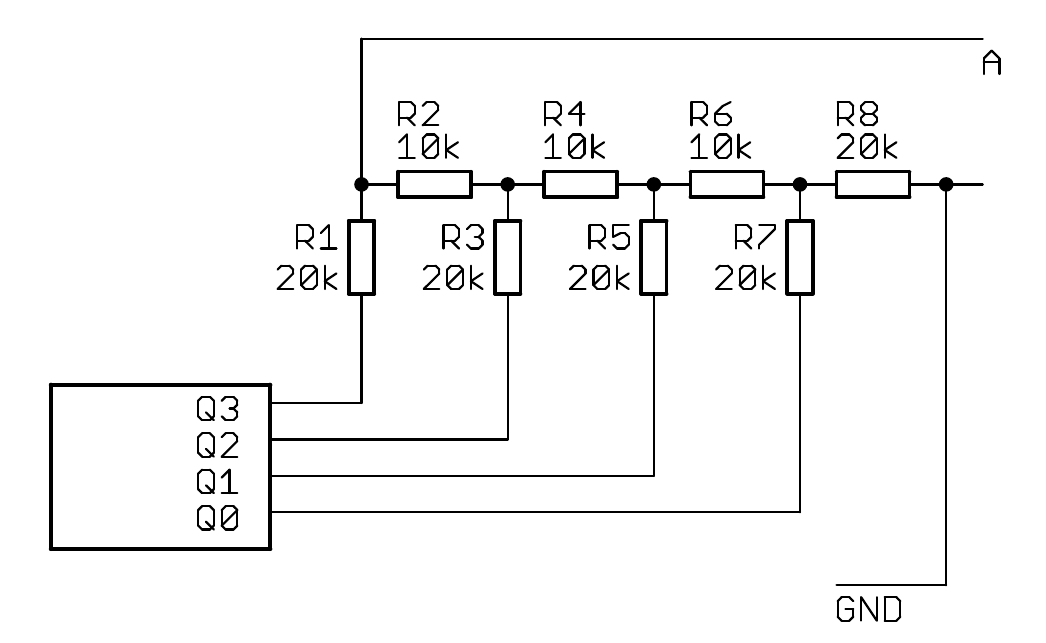
\includegraphics[ scale = 0.4]{auf_1_2.png}
  	\caption[Schaltplan für einen R-2R Netzwerk]{Schaltplan für einen R-2R Netzwerk\footnotemark}
  \label{fig:auf_1_2}
\end{figure}
\footnotetext{Abbildung entnommen von http://www.atlas.uni-wuppertal.de/$\sim$kind/ep11\_14.pdf am 18.01.2015}

\subsubsection*{Versuchsdurchführung}
%erklären, !was! wir machen, !warum! wir das machen und mit welchem ziel
%(wichtig) präzize erklären, wie bei dem versuch vorgegangen und was gemacht wurde

Das R-2R-Netzwerk wird mit acht Bits aufgebaut und das Ausgangssignal mit dem Oszilloskop untersucht.

\subsubsection*{Auswertung}
%zuerst !alle! errechneten werte entweder in ganzen sätzen aufzählen, oder in tabellen (übersichtlicher) dargestellen, sowie auf die verwendeten formeln verweisen (die referenzierung der formel kann in der überschrift stehen)
%kurz erwähnen (vor der tabelle), warum wir das ganze ausrechnen bzw. was wir dort ausrechnen
%danach histogramme und plots erstellen, wobei wenn möglich funktionen durch die plots gelegt werden (zur not können auch splines benutzt werden, was aber angegeben werden muss)
%bei fits immer die funktion und das reduzierte chiquadrat mit angegeben, wobei auf verständlichkeit beim entziffern der zehnerpotenzen geachtet werden muss z.b. f(x)=(wert+-fehler)\cdot10^{irgendeine zahl}\cdot x + (wert+-fehler)\cdot10^{irgendeine zahl}
%bei jedem fit erklären, nach welchem zusammenhang gefittet wurde und warum!
%bei plots darauf achten, dass die achsenbeschriftung (auch die tics) die richtige größe haben und die legende im plot nicht die messwerte verdeckt
%kurz die aufgabenstellung abhandeln
%2-----------------------------------------------2

Für den Zeitleichenverlauf wird wie im Teil zuvor eine Treppen-artiger Verlauf erwartet. Dabei ist die Auflösung höher da die Ausgangsspannung nach Gleichung \ref{eqn:binaer_2} bestimmt wird. Die Höhe einer Stufe ergibt sich mit $\frac{\text{U}_0}{2^\text{n}}$. In dem verwendetem Aufbau entspricht dies einer Stufenhöhe von einem 256-stel. Der Verlauf auf dem Oszilloskop ist in Abbildung \ref{fig:1_2_1} zu sehen. Aufgrund der hohen Auflösung sind die einzelnen Stufen nicht mehr zu erkennen.

\begin{figure}[H] 
  \centering 	
    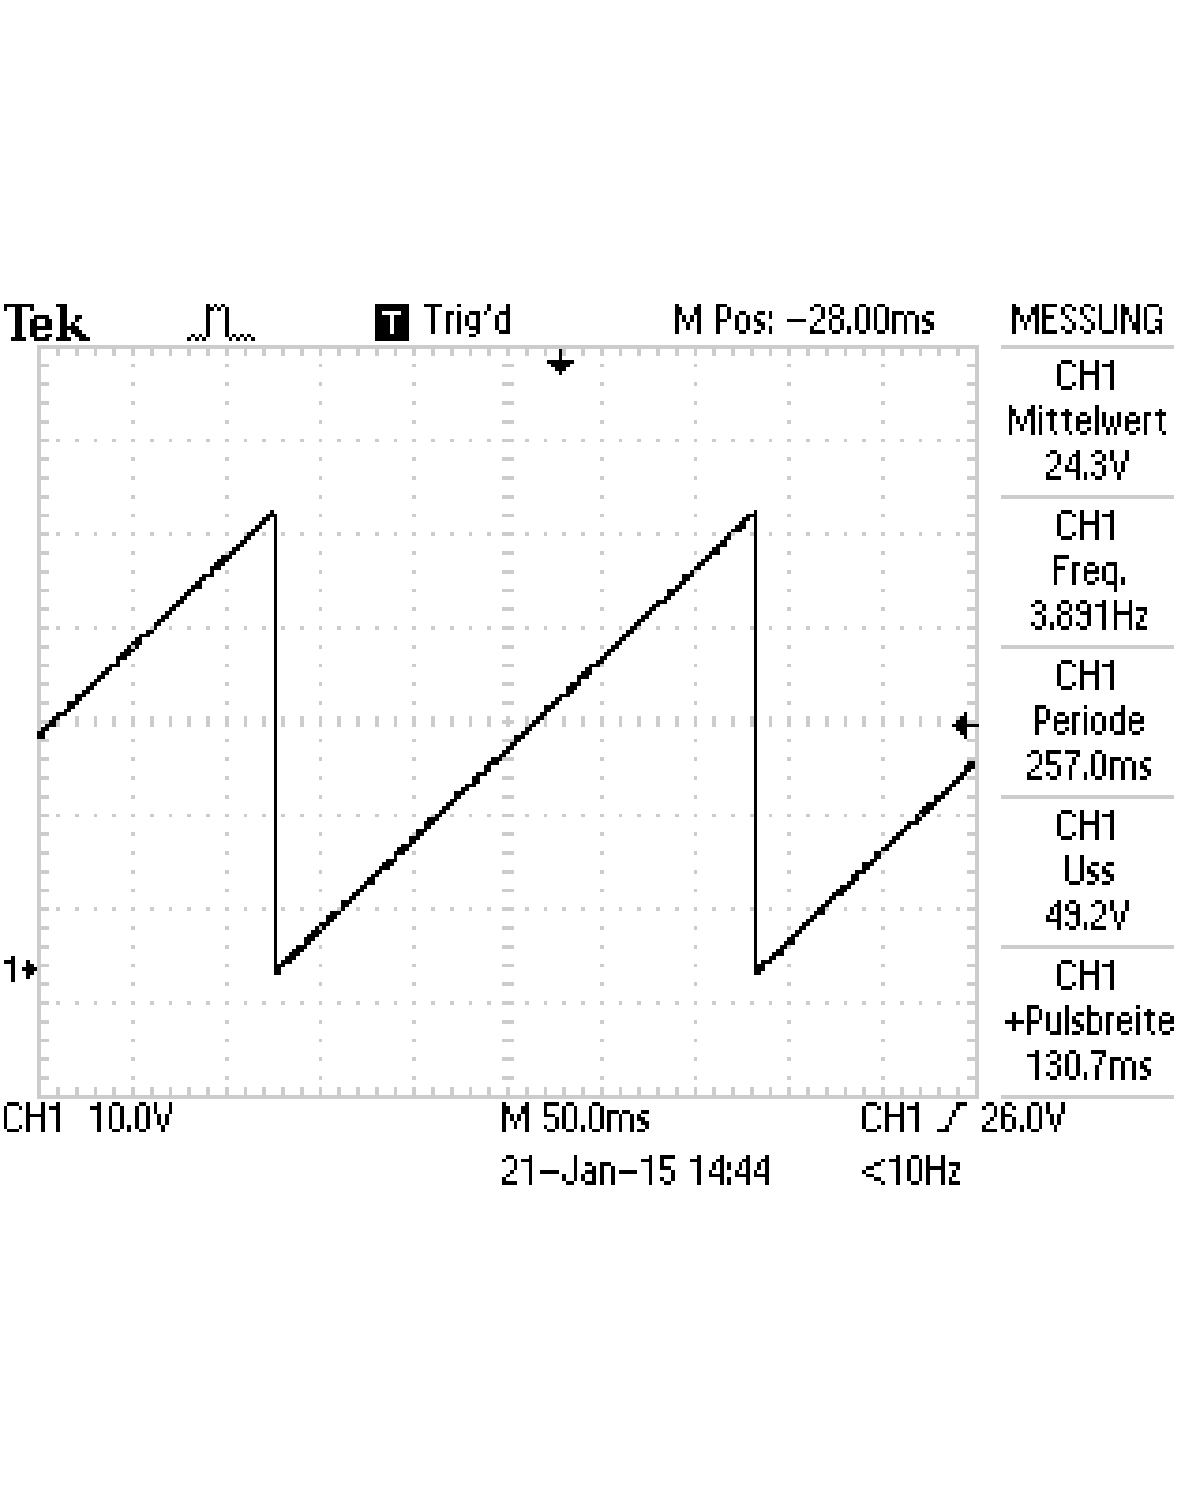
\includegraphics[trim = 0mm 50mm 0mm 50mm, clip, scale = 0.4]{1_2_1.pdf}
  	\caption[Aufnahme der Ausgangsspannung]{Aufnahme der Ausgangsspannung} 
  \label{fig:1_2_1}
\end{figure}
 

\subsubsection*{Diskussion}
%(immer) die gemessenen werte und die bestimmten werte über die messfehler mit literaturwerten oder untereinander vergleichen
%in welchem fehlerintervall des messwertes liegt der literaturwert oder der vergleichswert?
%wie ist der relative anteil des fehlers am messwert und damit die qualität unserer messung?
%in einem satz erklären, wie gut unser fehler und damit unsere messung ist
%kurz erläutern, wie systematische fehler unsere messung beeinflusst haben könnten
%(wichtig) zum schluss ansprechen, in wie weit die ergebnisse mit der theoretischen vorhersage übereinstimmen
%--------------------------------------------------------------------------------------------
%falls tabellen mit den messwerten zu lang werden, kann die section mit den messwerten auch hinter der diskussion angefügt bzw. eine section mit dem anhang eingefügt werden.
%1-----------------------------------------------1

Beide Messungen sind wie erwartet verlaufen. Da für das R-2R Netzwerk nur ein 8 Bit großes Netzwerk zur Verfügung stand können auch nur die beiden 8 Bit großen ADC verglichen werden. Vergleicht man die beiden Aufnahmen, Abbildung \ref{fig:1_1_2} für das Binärnetzwerk und Abbildung \ref{fig:1_2_1} für das R-2R Netzwerk ist kein Unterschied zu erkennen. Theoretisch sollten sich mit dem R-2R Netzwerk bessere Ergebnisse erzielen lassen, da es kaum von der Fehlern der Widerstände abhängt.



\section{Umwandlung analoger in digitale Signale, ADC}
%kurz das ziel dieses versuchsteiles ansprechen, damit keine zwei überschriften direkt übereinander stehen!
%bei schwierigeren versuchen kann auch der theoretische hintergrund erläutert werden. (mit formeln, herleitungen und erklärungen)

In diesem Versuchsabschnitt werden verschiedene Analog-Digital-Converter mit Hilfe des Boards aus Versuch 10 gebaut.

\subsection{ADC mit Zählverfahren und mit Approximationsverfahren}
%kurz das ziel dieses versuchsteiles ansprechen, damit keine zwei überschriften direkt übereinander stehen!
%bei schwierigeren versuchen kann auch der theoretische hintergrund erläutert werden. (mit formeln, herleitungen und erklärungen)

In diesem Versuchsteil wird ein ADC mit dem Zählverfahren und einer mit Apporximatoinsverfahren gebaut.

Der ADC mit Zählverfahren verwendet einen Binärzähler und ein R-2R Netzwerk um die Referenzspannung zu erzeugen. Der Stand des Binärzählers wird gespeichert, wenn der Komparator eine 0 ausgibt. Das Bitmuster des Zählers ist die Digitalisierung des analogen Signals. Der Nachteil des Verfahrens ist, dass der Aufwand zur Digitalisierung des Signals $\mathcal O(2^n)$ beträgt.

Der ADC mit Apporximatoinsverfahren bestehe aus einer Steuereinheit, einem R-2R Netzwerk und einem Komparator. Die Steuereinheit schaltet die Referenzspannung auf den halben Maximalwert. Wenn der Ausgang des Komparators auf 1 eins geht, wird die Referenzspannung auf $\frac{3}{4}$ der Maximalspannung gesetzt. Falls der Ausgang des Komparators auf 0 steht wird das aktuelle Bit auf 0 gesetzt und die Referenzspannung auf $\frac{1}{4}$ der Maximalspannung gesetzt. Der Vorteil dieses Verfahren ist, dass es wesentlich schneller als der ADC mit Zählverfahren ist. Der Aufwand beträgt $\mathcal O(n)$.

\subsubsection*{Verwendete Geräte}
%(immer) eine skizze oder ein foto einfügen, die geräte/materialien !nummerieren! und z.b. eine legende dazu schreiben, besser wäre es das ganze in einem Fließtext gut zu beschreiben.
%falls am anfang des versuches nicht klar ist, was alles verwendet wird, wenn möglich erst am ende ein großes foto von den verwendeten materialien machen!\\

Es werden das Board aus Versuch 10, ein Zusatzboard, ein Oszilloskop und ein Netzgerät verwendet.


\subsubsection*{Versuchsaufbau}
%skizze zum versuchsaufbau (oder foto) einfügen,   es muss erklärt werden wie das ganze funktioniert und welche speziellen einstellungen verwendet wurden (z.b. welche knöpfe an den geräten für die messung verdreht wurden)

Der Versuchsaufbau besteht aus dem Board von Versuch 10 und einem neuem Zusatzboard, in dem alle notwendigen Komponenten integriert sind.

\begin{figure}[H] 
  \centering 	
    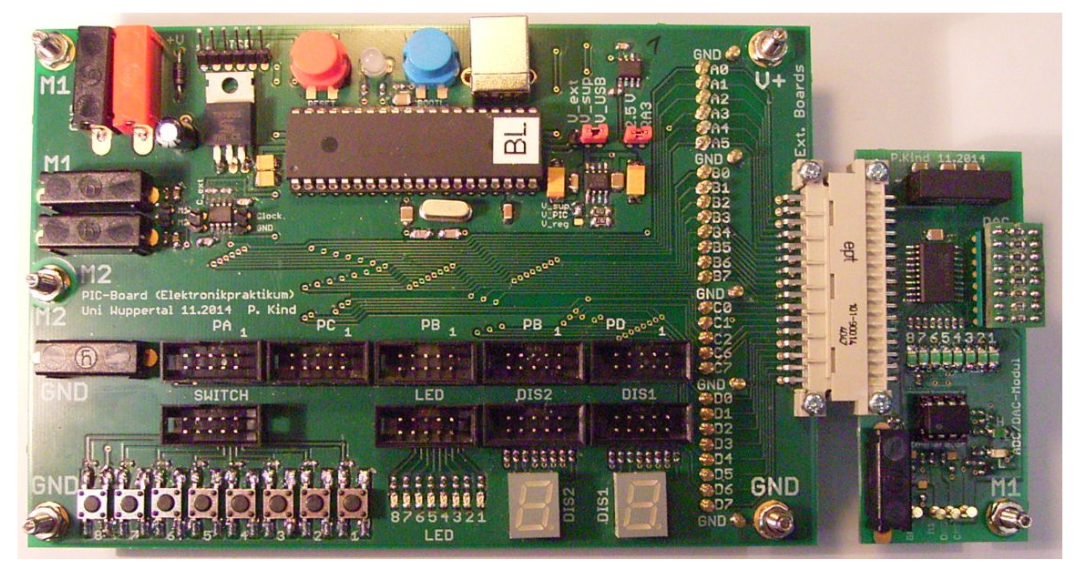
\includegraphics[ scale = 0.4]{auf_4.png}
  	\caption[Board und Zusatzborad]{Board und Zusatzborad\footnotemark}
  \label{fig:auf_2}
\end{figure}
\footnotetext{Abbildung entnommen von http://www.atlas.uni-wuppertal.de/$\sim$kind/ep11\_14.pdf am 18.01.2015}

\subsubsection*{Versuchsdurchführung}
%erklären, !was! wir machen, !warum! wir das machen und mit welchem ziel
%(wichtig) präzize erklären, wie bei dem versuch vorgegangen und was gemacht wurde

Das Zusatzboard wird an das Board angeschlossen, dies geschieht über einen seriellen Anschluss. Das vorgeschriebene Programm, zum messen der Daten wird auf das Board geladen. Danach wird die zu messende Spannung an M1 angeschlossen. Die Funktionalität wird untersucht, indem verschiedene Steuerzeichen (siehe nachfolgende Tabelle) an den Mikrocontroller geschickt werden. Dann werden unterschiedliche Spannungen eingestellt und die Ausgangssignale mit dem Oszilloskop beobachtet. Das Bitmuster wird jeweils abgelesen und notiert. Der Vorgang wird für das Zählverfahren und das Approximationsverfahren durchgeführt. Im nachfolgenden noch die Tabelle mit den Befehlen

\begin{itemize}
\item	?: Mikrocontroller meldet E-Prak Bergische Universität Wuppertal 2011“

\item	v: Mikrocontroller meldet Versionsnummer des Programms (V. PIC-Eval-Board for EP 1.2011)

\item	t: Mikrocontroller meldet OK“(Test der Verbindung)

\item	i: Mikrocontroller führt eine Messung nach dem Zählverfahren aus (iterativ, 10 ms Verzögerung)

\item	s: Mikrocontroller führt eine Messung nach dem Approximationsverfahren aus (sukzessiv, 10 ms Verzögerung)

\item	a: Mikrocontroller führt eine Messung nach dem Approximationsverfahren aus (sukzessiv durch Tasterfunktion an Port A0 mit 300 ms Verzögerung zum Entprellen)

\item	bxx: Gibt das Binärmuster xx (xx= hexadezimale Zahl von 00 bis ff) am Port B aus. Zum Beispiel b00 liefert 00000000, b01 liefert 00000001, b0f liefert 00001111 und bff liefert 11111111

\end{itemize}

\subsection{Messwerte}

\begin{table}[htbp]
\begin{center}
\begin{tabular}{|r|l|r|r|l|}
\hline
\multicolumn{1}{|l|}{Spannung/V} & Hex & \multicolumn{1}{l|}{Decimal} & \multicolumn{1}{l|}{Erwartet Binärwerte} & LEDs \\ \hline
0,5 & 1E & 30 & 11110 & 0b00011110 \\ \hline
1 & 39 & 57 & 111001 & 0b00111001 \\ \hline
1,5 & \multicolumn{1}{r|}{55} & 85 & 1010101 & 0b01010101 \\ \hline
2 & 6F & 111 & 1101111 & 0b01101110 \\ \hline
2,5 & \multicolumn{1}{r|}{89} & 137 & 10001001 & 0b10001001 \\ \hline
3 & A3 & 163 & 10100011 & 0b10100011 \\ \hline
3,5 & BD & 189 & 10111101 & 0b10111101 \\ \hline
4 & D5 & 213 & 11010101 & 0b11010101 \\ \hline
4,5 & EF & 239 & 11101111 & 0b11101111 \\ \hline
5 & FF & 255 & 11111111 & 0b11111111 \\ \hline
\end{tabular}
\end{center}
\caption{Messung zum Zählverfahren}
\label{tab:zaehl}
\end{table}

\begin{table}[htbp]
\begin{center}
\begin{tabular}{|r|l|r|r|l|}
\hline
\multicolumn{1}{|l|}{Spannung/V} & Hex & \multicolumn{1}{l|}{Decimal} & \multicolumn{1}{l|}{Erwartet Binärwerte} & LEDs \\ \hline
0,5 & 1F & 31 & 11111 & 0b00011111 \\ \hline
1 & \multicolumn{1}{r|}{38} & 56 & 111000 & 0b00111000 \\ \hline
1,5 & 4F & 79 & 1001111 & 0b01001111 \\ \hline
2 & 6F & 111 & 1101111 & 0b01101111 \\ \hline
2,5 & \multicolumn{1}{r|}{87} & 135 & 10000111 & 0b10000111 \\ \hline
3 & A0 & 160 & 10100000 & 0b10100000 \\ \hline
3,5 & BE & 190 & 10111110 & 0b10111110 \\ \hline
4 & D8 & 216 & 11011000 & 0b11011000 \\ \hline
4,5 & EF & 239 & 11101111 & 0b11101111 \\ \hline
5 & FF & 255 & 11111111 & 0b11111111 \\ \hline
\end{tabular}
\end{center}
\caption{Messung zum Approximationsverfahren}
\label{tab:approx}
\end{table}



\subsubsection*{Auswertung}
%zuerst !alle! errechneten werte entweder in ganzen sätzen aufzählen, oder in tabellen (übersichtlicher) dargestellen, sowie auf die verwendeten formeln verweisen (die referenzierung der formel kann in der überschrift stehen)
%kurz erwähnen (vor der tabelle), warum wir das ganze ausrechnen bzw. was wir dort ausrechnen
%danach histogramme und plots erstellen, wobei wenn möglich funktionen durch die plots gelegt werden (zur not können auch splines benutzt werden, was aber angegeben werden muss)
%bei fits immer die funktion und das reduzierte chiquadrat mit angegeben, wobei auf verständlichkeit beim entziffern der zehnerpotenzen geachtet werden muss z.b. f(x)=(wert+-fehler)\cdot10^{irgendeine zahl}\cdot x + (wert+-fehler)\cdot10^{irgendeine zahl}
%bei jedem fit erklären, nach welchem zusammenhang gefittet wurde und warum!
%bei plots darauf achten, dass die achsenbeschriftung (auch die tics) die richtige größe haben und die legende im plot nicht die messwerte verdeckt
%kurz die aufgabenstellung abhandeln
%2-----------------------------------------------2

Erwartet wird ein Treppen-artiger verlauf, welchen als solche, aufgrund der hohen Auflösung nicht direkt zu erkennen sein sollt. 

Bei dem Aufbau mit dem Zählverfahren war das hochgezählt der LEDs, bis die Spannung von 2 Volt erreicht wurde zu beobachten. Der Verlauf auf dem Oszilloskop ist in Abbildung \ref{fig:2_1_2V} zu sehen die untere Kurve ist das Signal des Komparators und die obere Kurve ist das Signal der Vergleichsspannung.

\begin{figure}[H]
  \centering 	
    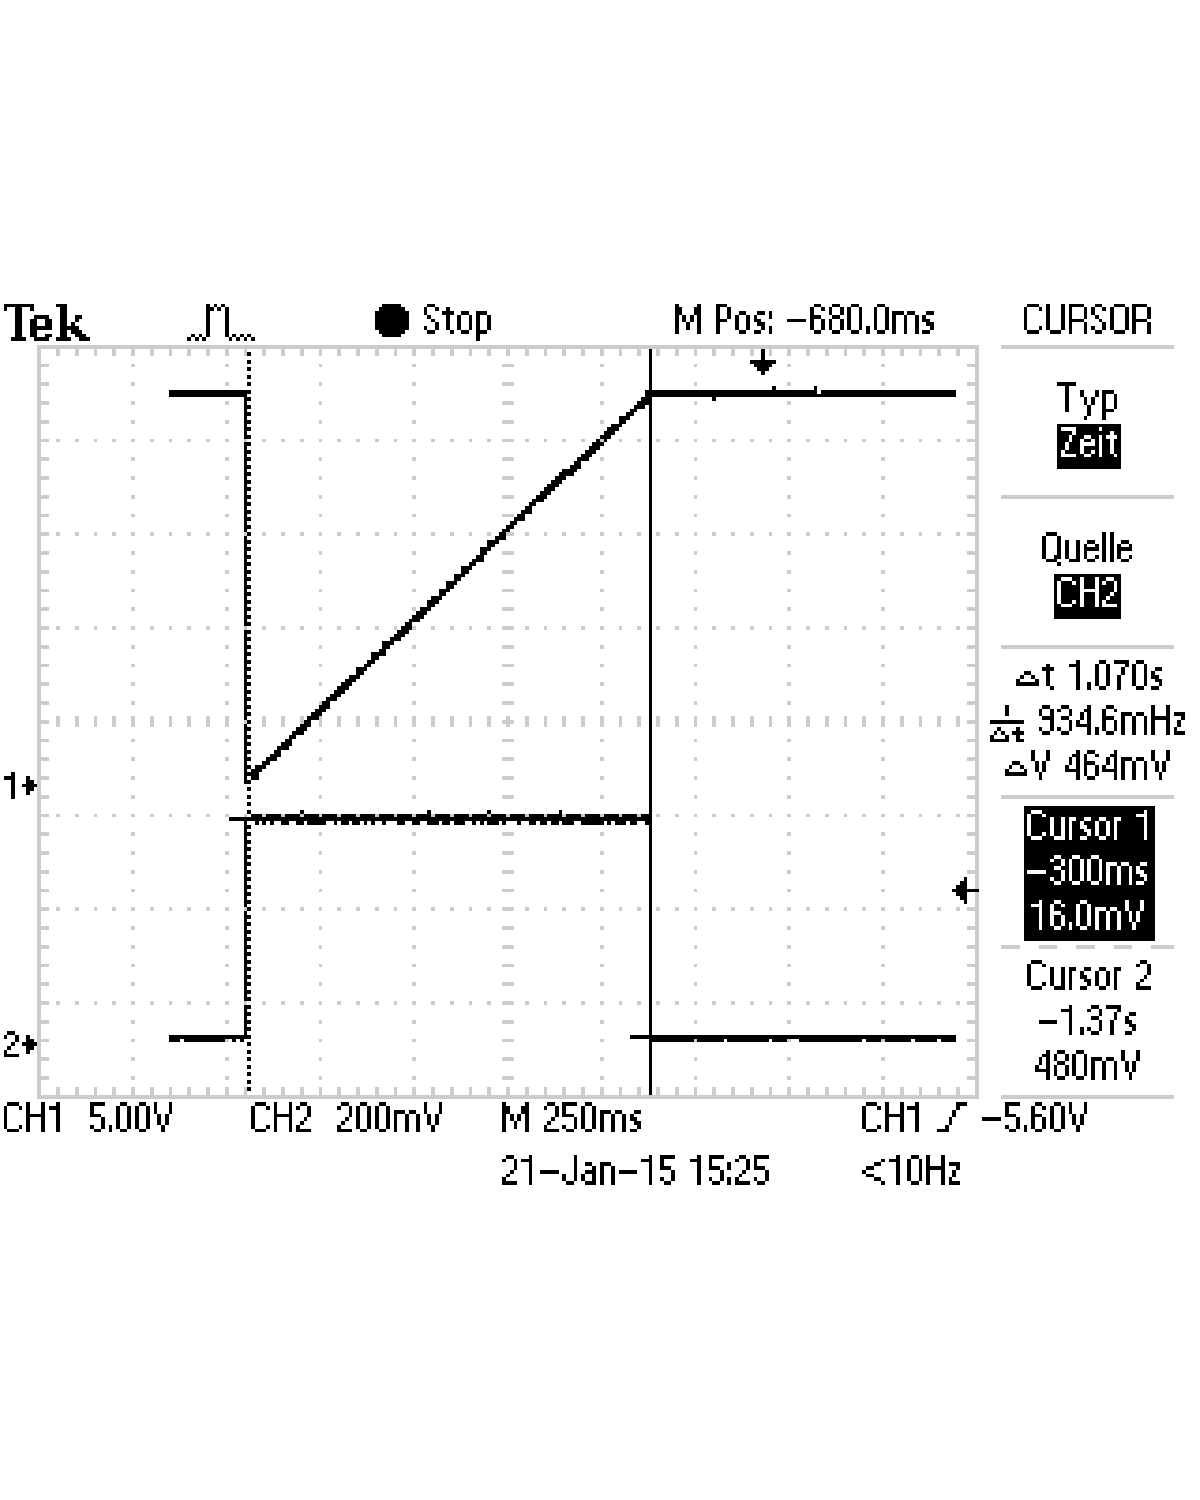
\includegraphics[trim = 0mm 50mm 0mm 50mm, clip, scale = 0.4]{2_1_4V.pdf}
  	\caption[Aufnahme der Ausgangs- und Komparatorspannung für eine Eingangssignal von 2V]{Aufnahme der Ausgangs- und Komparatorspannung für eine Eingangssignal von 2V} 
  \label{fig:2_1_4V}
\end{figure}

In Abbildung \ref{fig:2_1_2V} ist der Verlauf der Referenzspannung und der Komparatorspannung für die Umwandlung eines 4V Signals in ein Digitalesssignal dargestellt. An der Zeitauflösung ist zu sehen, das dass Umwandeln länger dauert als das Umwandeln des 2V Signals.

\begin{figure}[H]
  \centering 	
    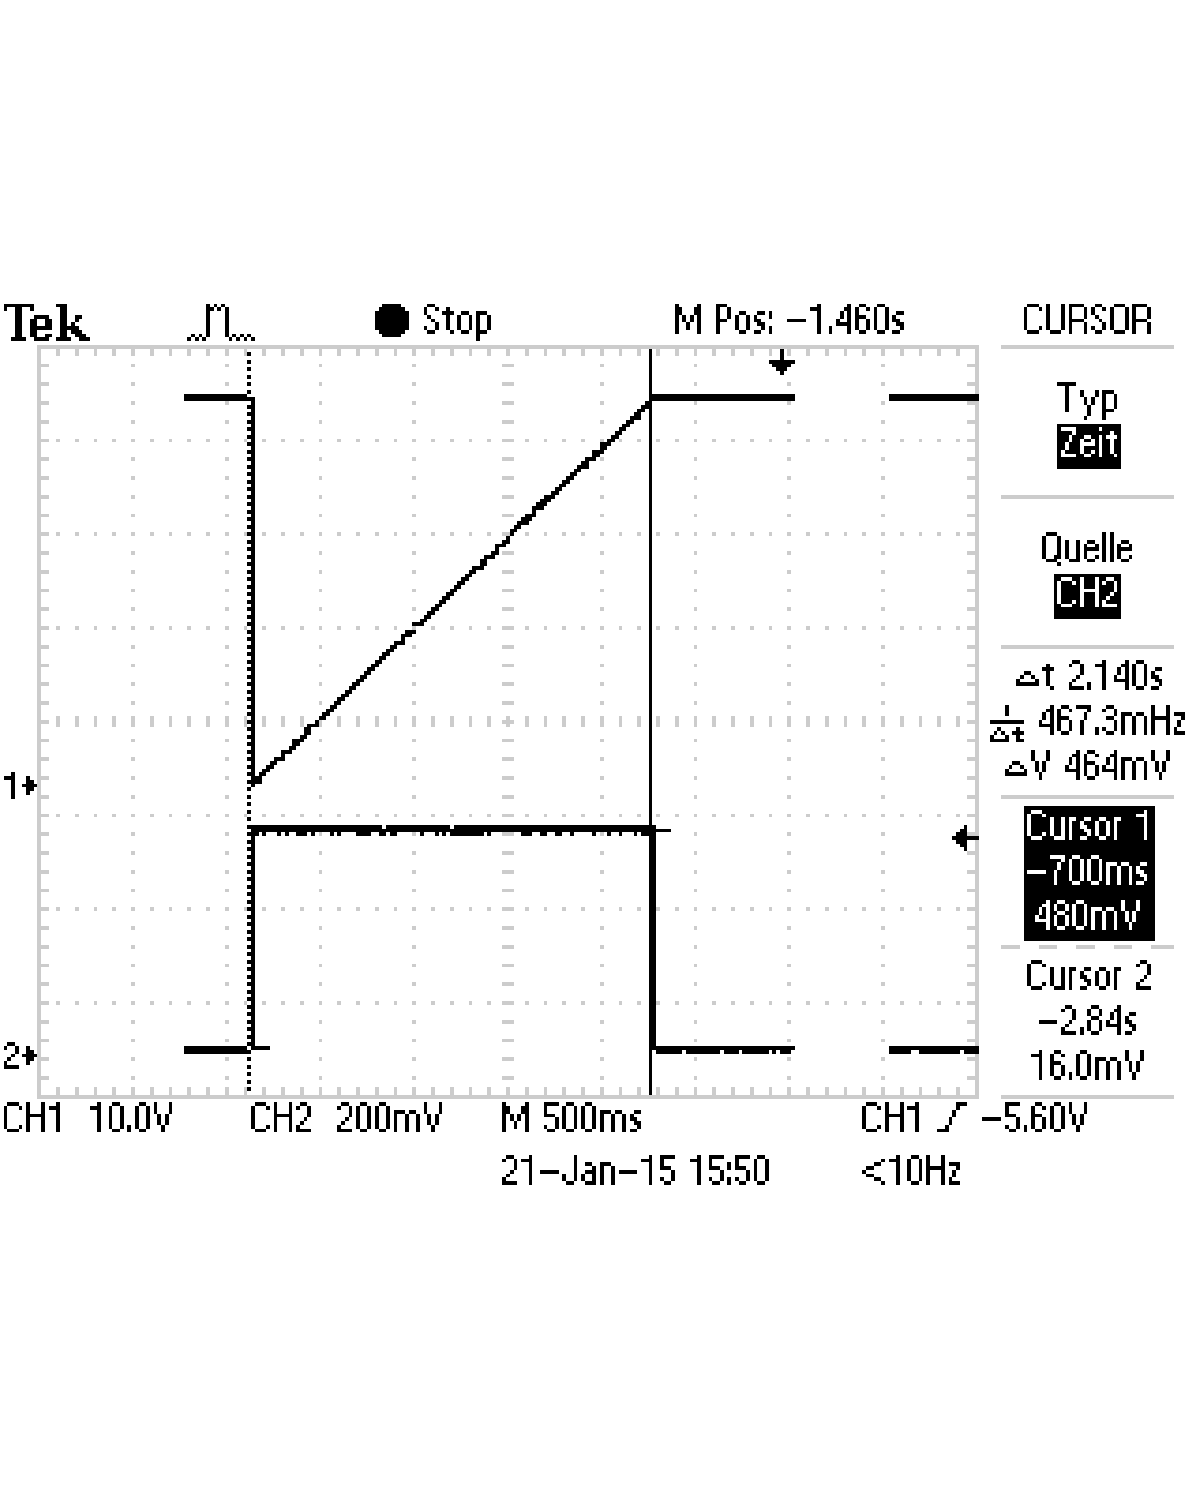
\includegraphics[trim = 0mm 50mm 0mm 50mm, clip, scale = 0.4]{2_1_2V.pdf}
  	\caption[Aufnahme der Ausgangs- und Komparatorspannung für eine Eingangssignal von 4V]{Aufnahme der Ausgangs- und Komparatorspannung für eine Eingangssignal von 4V} 
  \label{fig:2_1_2V}
\end{figure}

Bei der Umwandlung eines 2V Signals mit dem Approximationsverfahren ergab sich der Verlauf in Abbildung \ref{fig:2_2_2V} zu sehen. Die untere Kurve ist das Signal des Komparators und die obere Kurve ist das Signal der Steuereinheit.

\begin{figure}[H]
  \centering 	
    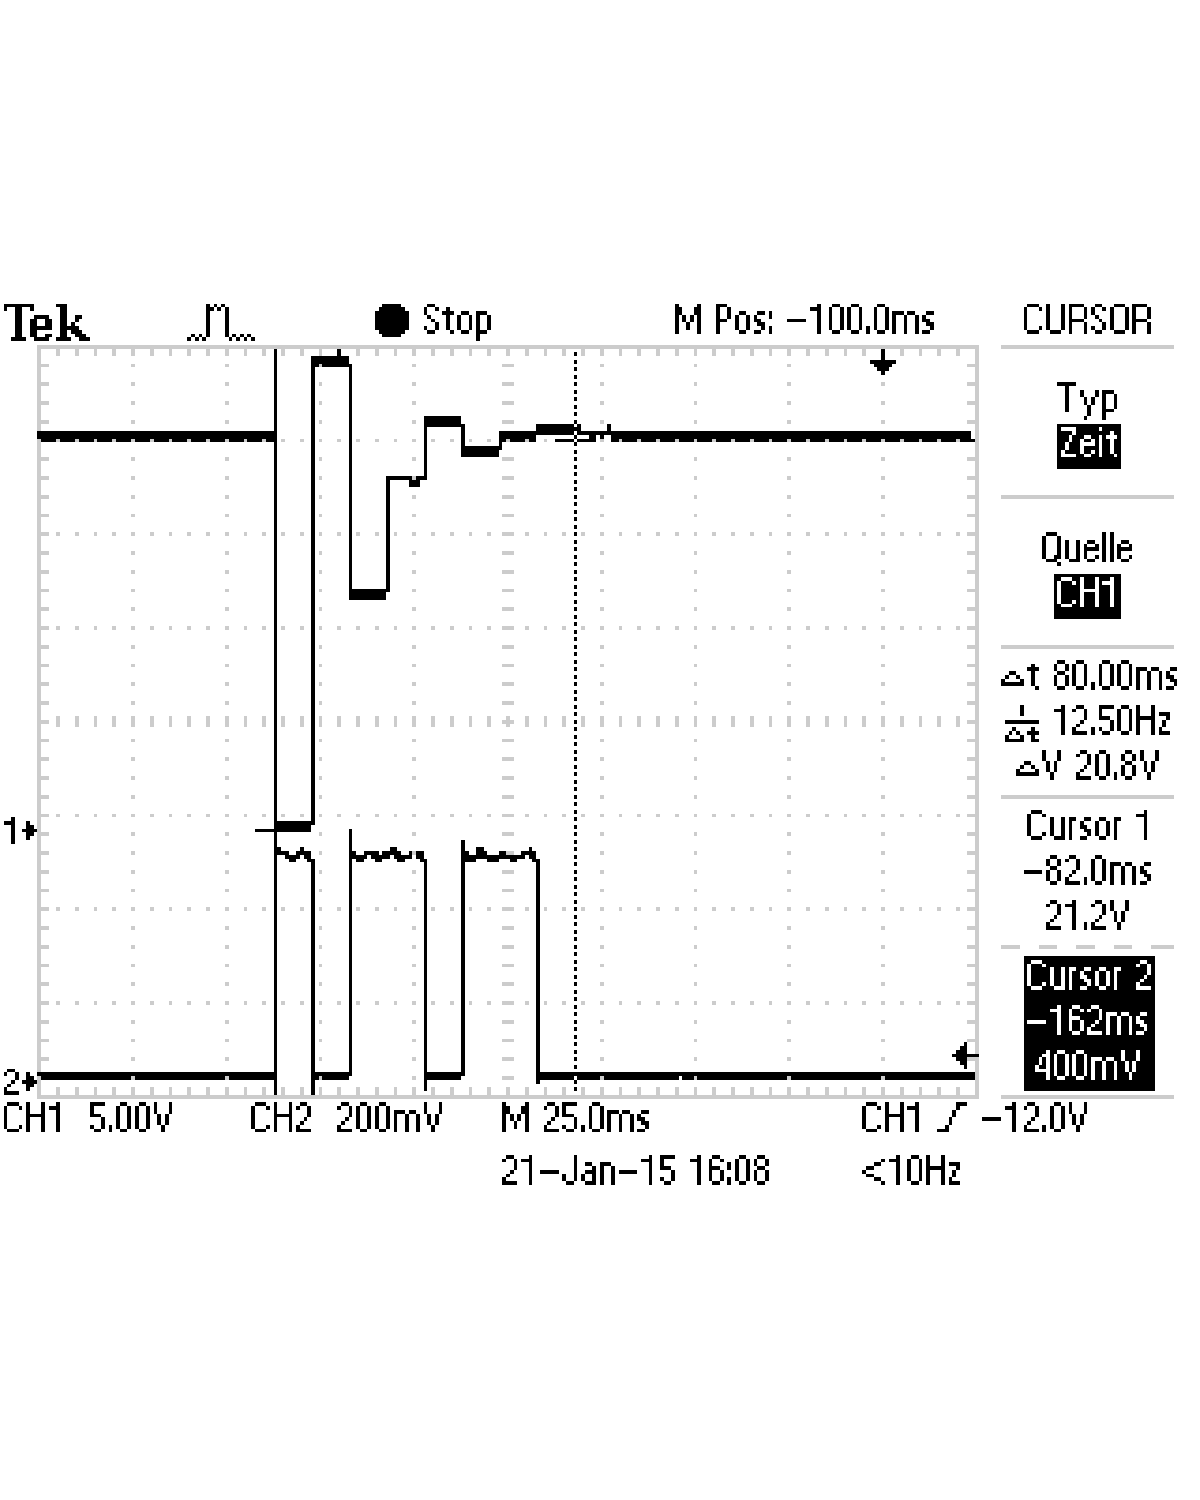
\includegraphics[trim = 0mm 50mm 0mm 50mm, clip, scale = 0.4]{2_2_2V.pdf}
  	\caption[Aufnahme der Ausgangs- und Komparatorspannung für eine Eingangssignal von 2V]{Aufnahme der Ausgangs- und Komparatorspannung für eine Eingangssignal von 2V} 
  \label{fig:2_2_2V}
\end{figure}

Die Umwandelung eines 4V Signals ist in Abbildung \ref{fig:2_2_4V} zu sehen. Die ben

\begin{figure}[H]
  \centering 	
    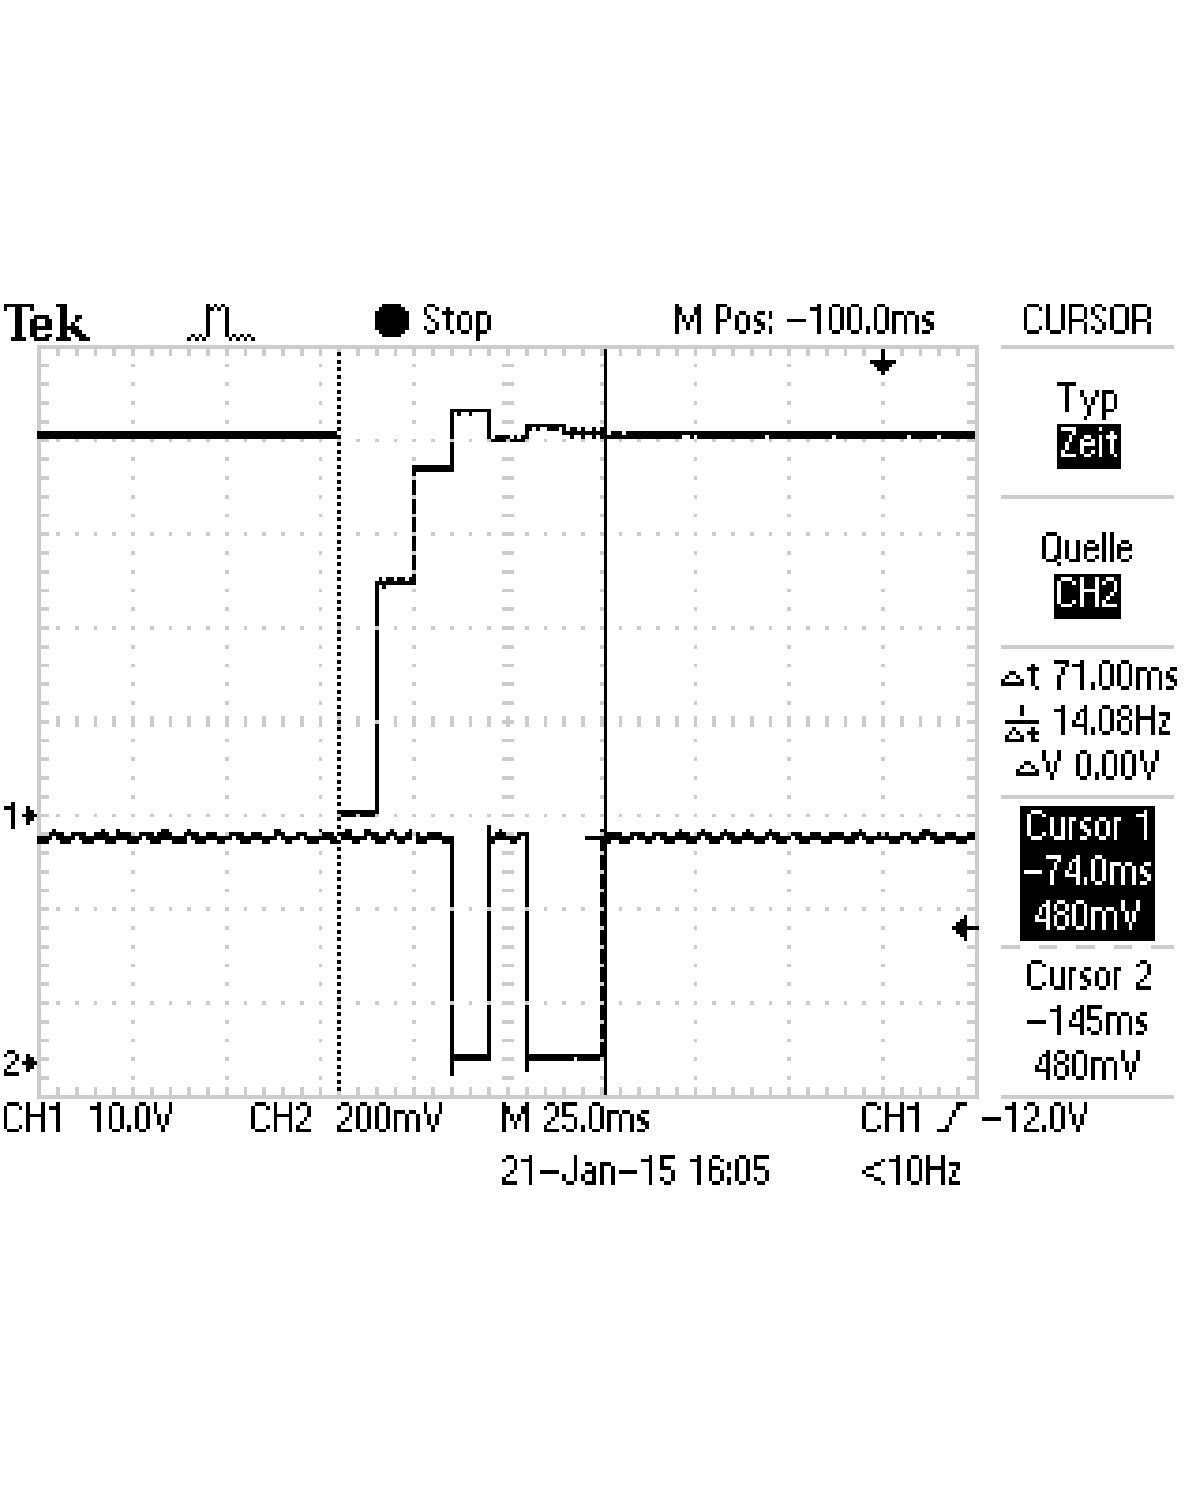
\includegraphics[trim = 0mm 50mm 0mm 50mm, clip, scale = 0.4]{2_2_4V.pdf}
  	\caption[Aufnahme der Ausgangs- und Komparatorspannung für eine Eingangssignal von 4V]{Aufnahme der Ausgangs- und Komparatorspannung für eine Eingangssignal von 4V} 
  \label{fig:2_2_4V}
\end{figure}

Beim Steuern des Approximationsverfahren mit einem Taster war zu erkennen, das nach jedem Drücken des Tasters die Stufe der Referenzspannung kleiner wurde.

\subsubsection*{Diskussion}
%(immer) die gemessenen werte und die bestimmten werte über die messfehler mit literaturwerten oder untereinander vergleichen
%in welchem fehlerintervall des messwertes liegt der literaturwert oder der vergleichswert?
%wie ist der relative anteil des fehlers am messwert und damit die qualität unserer messung?
%in einem satz erklären, wie gut unser fehler und damit unsere messung ist
%kurz erläutern, wie systematische fehler unsere messung beeinflusst haben könnten
%(wichtig) zum schluss ansprechen, in wie weit die ergebnisse mit der theoretischen vorhersage übereinstimmen
%--------------------------------------------------------------------------------------------
%falls tabellen mit den messwerten zu lang werden, kann die section mit den messwerten auch hinter der diskussion angefügt bzw. eine section mit dem anhang eingefügt werden.
%1-----------------------------------------------1




\section{Zeit- und Frequenzmessung}
%kurz das ziel dieses versuchsteiles ansprechen, damit keine zwei überschriften direkt übereinander stehen!
%bei schwierigeren versuchen kann auch der theoretische hintergrund erläutert werden. (mit formeln, herleitungen und erklärungen)

In diesem Versuchsabschnitt werden eine Stoppuhr und ein Frequenzzähler gebaut.

\subsection{Bau einer Stoppuhr}
%kurz das ziel dieses versuchsteiles ansprechen, damit keine zwei überschriften direkt übereinander stehen!
%bei schwierigeren versuchen kann auch der theoretische hintergrund erläutert werden. (mit formeln, herleitungen und erklärungen)

In diesem Versuchsteil wird eine Stoppuhr gebaut.

\subsubsection*{Verwendete Geräte}
%(immer) eine skizze oder ein foto einfügen, die geräte/materialien !nummerieren! und z.b. eine legende dazu schreiben, besser wäre es das ganze in einem Fließtext gut zu beschreiben.
%falls am anfang des versuches nicht klar ist, was alles verwendet wird, wenn möglich erst am ende ein großes foto von den verwendeten materialien machen!\\

Es werden ein Taktzähler Typ 4040, ein Kondensator, Widerstände, ein NAND-Gatter, LEDs und eine Spannungsquelle verwendet.

\subsubsection*{Versuchsaufbau}
%skizze zum versuchsaufbau (oder foto) einfügen,   es muss erklärt werden wie das ganze funktioniert und welche speziellen einstellungen verwendet wurden (z.b. welche knöpfe an den geräten für die messung verdreht wurden)

Schaltplan zum Aufbau der Stoppuhr.

\begin{figure}[H] 
  \centering 	
    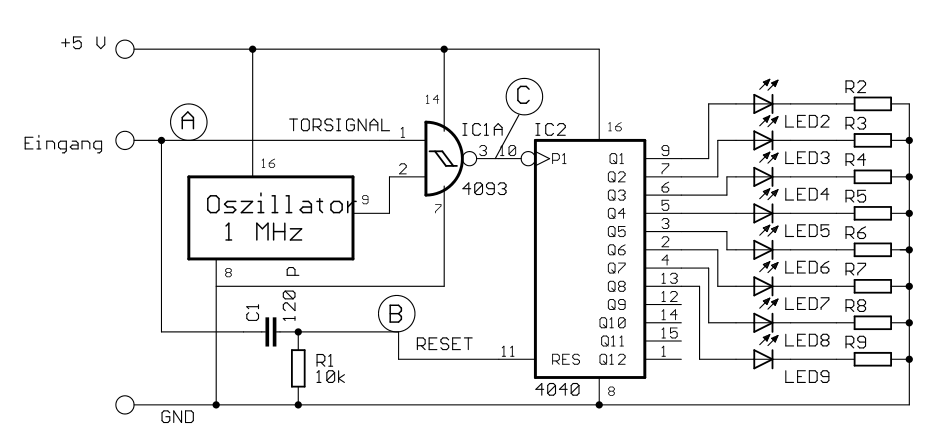
\includegraphics[ scale = 0.4]{auf_5.png}
  	\caption[Schaltplan der Stoppuhr]{Schaltplan der Stoppuhr\footnotemark}
  \label{fig:auf_3}
\end{figure}
\footnotetext{Abbildung entnommen von http://www.atlas.uni-wuppertal.de/$\sim$kind/ep11\_14.pdf am 18.01.2015}

\subsubsection*{Versuchsdurchführung}
%erklären, !was! wir machen, !warum! wir das machen und mit welchem ziel
%(wichtig) präzize erklären, wie bei dem versuch vorgegangen und was gemacht wurde

Nachdem Schaltung \ref{fig:auf_3} aufgebaut wurde, wird ein Eingangssignal mit einer Amplitude von 5V (Rechteckpulse mit kurzer Signalbreite und langen Pausen) eingestellt. Die Frequenz des Funktionsgenerators wird so gewählt, das die Maximalzeit, welche mit der Stoppuhr gemessen werden kann, nicht überstiegen wird. Danach wird das Bitmuster der LEDs gelesen und umgerechnet. Die Impulse des Funktionsgenerators werden dann mit dem Oszilloskop untersucht um nochmal die Pulsdauer zu bestimmen, welche mit den gemessenen Werten verglichen werden soll.

\subsubsection*{Auswertung}
%zuerst !alle! errechneten werte entweder in ganzen sätzen aufzählen, oder in tabellen (übersichtlicher) dargestellen, sowie auf die verwendeten formeln verweisen (die referenzierung der formel kann in der überschrift stehen)
%kurz erwähnen (vor der tabelle), warum wir das ganze ausrechnen bzw. was wir dort ausrechnen
%danach histogramme und plots erstellen, wobei wenn möglich funktionen durch die plots gelegt werden (zur not können auch splines benutzt werden, was aber angegeben werden muss)
%bei fits immer die funktion und das reduzierte chiquadrat mit angegeben, wobei auf verständlichkeit beim entziffern der zehnerpotenzen geachtet werden muss z.b. f(x)=(wert+-fehler)\cdot10^{irgendeine zahl}\cdot x + (wert+-fehler)\cdot10^{irgendeine zahl}
%bei jedem fit erklären, nach welchem zusammenhang gefittet wurde und warum!
%bei plots darauf achten, dass die achsenbeschriftung (auch die tics) die richtige größe haben und die legende im plot nicht die messwerte verdeckt
%kurz die aufgabenstellung abhandeln
%2-----------------------------------------------2

\begin{table}[htbp]
\begin{center}
\begin{tabular}{|r|l|}
\hline
\multicolumn{1}{|l|}{Spannung/V} & Binärmuster \\ \hline \hline
19,05 & 0b00010011 \\ \hline
66,89 & 0b11000011 \\ \hline
207,1 & 0b11001111 \\ \hline
\end{tabular}
\end{center}
\caption{Bitmuster in Abhängigkeit der Frequenz}
\label{tab:span}
\end{table}



\subsubsection*{Diskussion}
%(immer) die gemessenen werte und die bestimmten werte über die messfehler mit literaturwerten oder untereinander vergleichen
%in welchem fehlerintervall des messwertes liegt der literaturwert oder der vergleichswert?
%wie ist der relative anteil des fehlers am messwert und damit die qualität unserer messung?
%in einem satz erklären, wie gut unser fehler und damit unsere messung ist
%kurz erläutern, wie systematische fehler unsere messung beeinflusst haben könnten
%(wichtig) zum schluss ansprechen, in wie weit die ergebnisse mit der theoretischen vorhersage übereinstimmen
%--------------------------------------------------------------------------------------------
%falls tabellen mit den messwerten zu lang werden, kann die section mit den messwerten auch hinter der diskussion angefügt bzw. eine section mit dem anhang eingefügt werden.
%1-----------------------------------------------1





\subsection{Bau eines Frequenzzählers}
%kurz das ziel dieses versuchsteiles ansprechen, damit keine zwei überschriften direkt übereinander stehen!
%bei schwierigeren versuchen kann auch der theoretische hintergrund erläutert werden. (mit formeln, herleitungen und erklärungen)
In diesem Versuchsteil wird die Stoppuhr in einen Frequenzzähler umgebaut, welcher für einen vorgegebenen Zeitraum die Anzahl der am Eingang eintreffenden Impulse zählen soll.
\subsubsection*{Verwendete Geräte}
%(immer) eine skizze oder ein foto einfügen, die geräte/materialien !nummerieren! und z.b. eine legende dazu schreiben, besser wäre es das ganze in einem Fließtext gut zu beschreiben.
%falls am anfang des versuches nicht klar ist, was alles verwendet wird, wenn möglich erst am ende ein großes foto von den verwendeten materialien machen!\\
Es werden drei Taktzähler Typ 4040, ein Kondensator, zwei Widerstände, ein NAND-Gatter, LEDs, ein Oszillator, einen HAMEG-Funktionsgenerator und eine Spannungsquelle verwendet.
\subsubsection*{Versuchsaufbau}
%skizze zum versuchsaufbau (oder foto) einfügen,   es muss erklärt werden wie das ganze funktioniert und welche speziellen einstellungen verwendet wurden (z.b. welche knöpfe an den geräten für die messung verdreht wurden)
Schaltplan zum Aufbau eines Frequenzzählers.
\begin{figure}[H] 
  \centering 	
    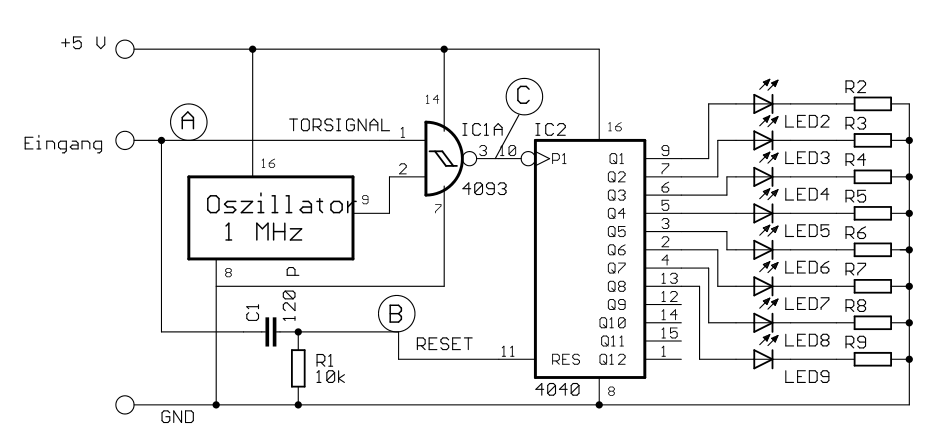
\includegraphics[ scale = 0.4]{auf_5.png}
  	\caption[Schaltplan des Frequenzzählers]{Schaltplan des Frequenzzählers\footnotemark}
  \label{fig:auf_3_2}
\end{figure}
\footnotetext{Abbildung entnommen von http://www.atlas.uni-wuppertal.de/$\sim$kind/ep11\_14.pdf am 18.01.2015}
\subsubsection*{Versuchsdurchführung}
%erklären, !was! wir machen, !warum! wir das machen und mit welchem ziel
%(wichtig) präzize erklären, wie bei dem versuch vorgegangen und was gemacht wurde
Die Stoppuhr wird zum Frequenzzähler umgebaut, indem das Torsignal vom Oszillator gewonnen wird. Zwischen Oszillator und NAND-Baustein werden zwei Zähler geschaltet, welche die Frequenz des Oszillators durch $2^{22}$ teilen (siehe Schaltung \ref{fig:auf_3_2}). Die Torzeit beträgt jetzt eine Sekunde (\unit[0,5]{Hz}), da der Oszillator mit einer Frequenz von \unit[2,09715]{MHz} arbeitet. Nachdem die Schaltung aufgebaut wurde, wird, nachdem mit dem Oszilloskop überprüft wurde, dass der Eingang ein Signal zwischen 0 und \unit[5]{V} liefert, eine Spannung von \unit[5]{V} angelegt und die Frequenz der Ausgangsimpulse des Funktionsgenerators gemessen. Die maximal Messbare Frequenz liegt bei genau \unit[4,096]{kHz}, daher muss das Eingangssignal passend dazu gewählt werden. Zum Schluss wird der Messwert mit der Anzeige am Funktionsgenerator verglichen.
\subsubsection*{Auswertung}
%zuerst !alle! errechneten werte entweder in ganzen sätzen aufzählen, oder in tabellen (übersichtlicher) dargestellen, sowie auf die verwendeten formeln verweisen (die referenzierung der formel kann in der überschrift stehen)
%kurz erwähnen (vor der tabelle), warum wir das ganze ausrechnen bzw. was wir dort ausrechnen
%danach histogramme und plots erstellen, wobei wenn möglich funktionen durch die plots gelegt werden (zur not können auch splines benutzt werden, was aber angegeben werden muss)
%bei fits immer die funktion und das reduzierte chiquadrat mit angegeben, wobei auf verständlichkeit beim entziffern der zehnerpotenzen geachtet werden muss z.b. f(x)=(wert+-fehler)\cdot10^{irgendeine zahl}\cdot x + (wert+-fehler)\cdot10^{irgendeine zahl}
%bei jedem fit erklären, nach welchem zusammenhang gefittet wurde und warum!
%bei plots darauf achten, dass die achsenbeschriftung (auch die tics) die richtige größe haben und die legende im plot nicht die messwerte verdeckt
%kurz die aufgabenstellung abhandeln
%2-----------------------------------------------2

\begin{table}[htbp]
\begin{center}
\begin{tabular}{|r|l|}
\hline
\multicolumn{1}{|l|}{Frequenz/Hz} & Binärmuster \\ \hline \hline
140 & 0b10001100 \\ \hline
86 & 0b01010110 \\ \hline
32 & 0b00100000 \\ \hline
8 & 0b00001000 \\ \hline
\end{tabular}
\end{center}
\caption{Bitmuster in Abhängigkeit der Frequenz}
\label{tab:frequ}
\end{table}




\subsubsection*{Diskussion}
%(immer) die gemessenen werte und die bestimmten werte über die messfehler mit literaturwerten oder untereinander vergleichen
%in welchem fehlerintervall des messwertes liegt der literaturwert oder der vergleichswert?
%wie ist der relative anteil des fehlers am messwert und damit die qualität unserer messung?
%in einem satz erklären, wie gut unser fehler und damit unsere messung ist
%kurz erläutern, wie systematische fehler unsere messung beeinflusst haben könnten
%(wichtig) zum schluss ansprechen, in wie weit die ergebnisse mit der theoretischen vorhersage übereinstimmen
%--------------------------------------------------------------------------------------------
%falls tabellen mit den messwerten zu lang werden, kann die section mit den messwerten auch hinter der diskussion angefügt bzw. eine section mit dem anhang eingefügt werden
%1-----------------------------------------------1


\section{Fazit}
%im fazit nochmal alles zusammenfassen und den verlauf der messung abschätzen
%gravierende sytematische probleme bei den messungen nochmal betonen und die wertigkeit unserer ergebnisse einordnen
\end{document}

